\chapter{Results}

Simulation results are presented in terms of success rate (section \ref{sec:results_success_rate}) and delay (section \ref{sec:results_delay}).

%--------------------------------------------------------------------------------------------------------
% 		Success Rate
%--------------------------------------------------------------------------------------------------------
\section{Success Rate}
\label{sec:results_success_rate}

As discussed in section \ref{sec:packetloss}, memory limit is the most important parameter affecting success rate. 
%TODO: more?

\subsection{Simulation 1}
\label{sec:results_success_scenario1}

The update success rate for the first simulation with one ferry and one gateway is shown in \ref{fig:result_sccess_sim1byseed_dss}.
Success rate is shown as a function of ferry memory capacity. 
Results for two separate seeds are shown since ferry movement, and hence delivery times and success rate, is heavily affected by randomness.
The spike in success rate shown for the first simulation (seed of 128) at a memory capacity of four is an artifact of this randomness.
It can be seen from this figure that success rate increases rapidly with memory capacity.
There is a leveling effect seen when memory capacity increases beyond 30.
Since there are ten source nodes each with three properties and the storage process is intelligent about keeping only the most current updates, no packets must be discarded (see section \ref{sec:algorithm}).
%	At this point
The fact that success rate never reaches 1, or 100\%, is an artifact of the limited simulation time.
Were the simulation to run forever and ferries to visit every source node, success rate would approach 1.

\begin{figure}[htbp]
    \begin{center}
    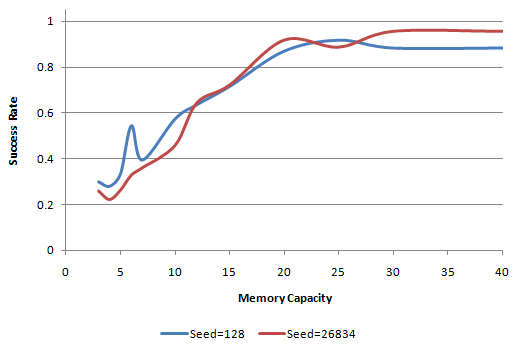
\includegraphics[width=0.8\textwidth]{images/result_sccess_sim1byseed_dss}
    \caption{Success Rate vs Memory Capacity - Simulation 1 (1 Ferry, 1 Gateway), Source Storage Disabled}
    \label{fig:result_sccess_sim1byseed_dss}
    \end{center}
\end{figure}

\subsection{Simulation 2}
\label{sec:results_success_s2}

The update success rate for second simulation, with two ferries and two gateways, is shown in figure \ref{fig:result_sccess_sim2byseed_dss}.
As in section \ref{sec:results_success_scenario1}, success rate is shown as a function of ferry memory capacity and results for two separate seeds are shown.
It can be seen that variability in the success rate between the two seed values is lower than the first scenario.
Increasing the number of ferries and gateways increases the likely hood a ferry will pass by the node and decreases variance.
%Something about gussians and decreasing variance.

\begin{figure}[htbp]
    \centering
    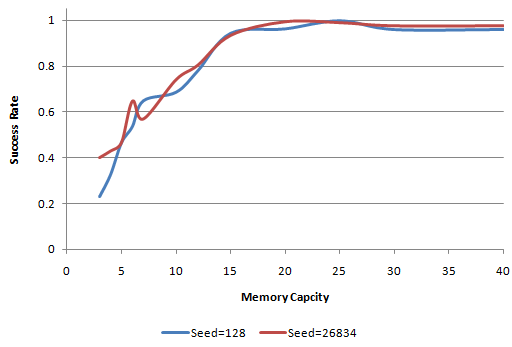
\includegraphics[width=0.8\textwidth]{images/result_sccess_sim2byseed_dss}
    \caption{Success Rate vs Memory Capacity - Simulation 2 (2 Ferries, 2 Gateways), Source Storage Disabled}
    \label{fig:result_sccess_sim2byseed_dss}
\end{figure}

\subsection{Comparison of Success Rate}

A comparison of success rate between simulations 1 and 2 is show in figure \ref{fig:result_sccess_bothsim_128_dss}.
It can be seen the additional ferry and gateway significantly increase success rate; this result is expected.
As discussed in section \ref{sec:results_success_scenario1}, the success rate should be 1 for memory capacities beyond 30. 
The fact that it is not is a result of limited simulation time.

\begin{figure}[htbp]
    \centering
    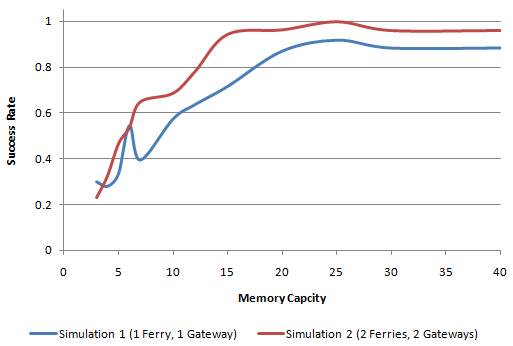
\includegraphics[width=0.8\textwidth]{images/result_sccess_bothsim_128_dss}
    \caption{Success Rate vs Memory Capacity - Simulation 1 and 2 , Seed of 128 and Source Storage Disabled}
    \label{fig:result_sccess_bothsim_128_dss}
\end{figure}

\subsection{Effect of Source Node Storage}

As discussed in section \ref{sec:source_node_storage}, source nodes can be configured to receive updates from ferries, store them and retransmit them; in essence, acting as stationary ferries.
The impact of enabling source node storage on success rate in simulation 2 can be seen in \ref{fig:result_sccess_sim2byss_128}.
%	TODO: reword
It can be seen that although success rate increased, the change was not drastic.
This result is somewhat expected given that there were only two ferries and all source nodes were relatively close to gateways.
It is expected that the impact of enabling source node storage would become more pronounced by increasing the number of ferries or increasing the distance between source nodes and gateways while keeping the relative spacing of source nodes constant
%	Terrible
%	TODO: Explain why
Enabling source node storage in simulation 1 was seen to have no impact on success rate.
This is expected as the algorithm used to discard packets in the presence of memory constrains would prevent a ferry re-storing up an update it had previously discarded.


%\begin{figure}[htbp]
%    \centering
%    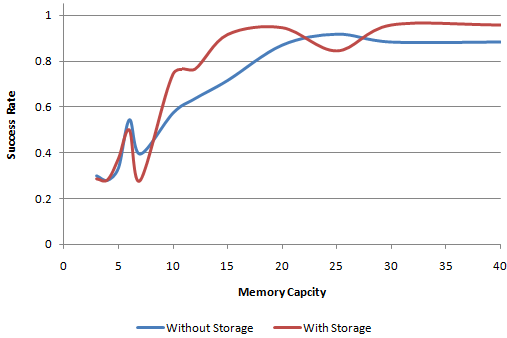
\includegraphics[width=0.8\textwidth]{images/result_sccess_sim1byss_128}
%    \caption{Effect of Source Node Storage - Success Rate vs Memory Capacity - Simulation 1, Seed of 128}
%    \label{fig:result_sccess_sim1byss_128}
%\end{figure}

\begin{figure}[htbp]
    \centering
    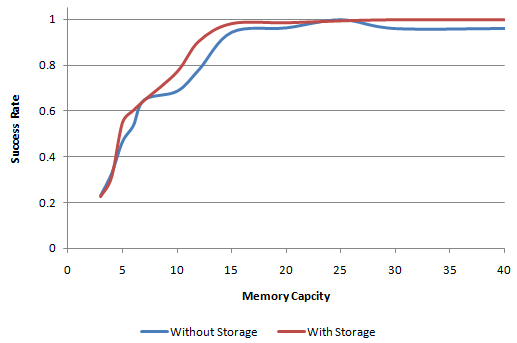
\includegraphics[width=0.8\textwidth]{images/result_sccess_sim2byss_128}
    \caption{Effect of Source Node Storage - Success Rate vs Memory Capacity - Simulation 2, Seed of 128}
    \label{fig:result_sccess_sim2byss_128}
\end{figure}


%--------------------------------------------------------------------------------------------------------
% 		Delay
%--------------------------------------------------------------------------------------------------------
\section{Delay}
\label{sec:results_delay}
The time between a property value changing and when that change is registered by the gateway is of interest and examined.
Delay is presented as a cumulative distribution function.
A CDF was chosen over a PDF as it is more meaningful in the presence of random ferry movement.
%
It is important to note that delay results presented here only account for updates successfully delivered.
Updates lost as defined in section \ref{sec:packetloss}, with the exception of the very last update, do not count towards the measured delay.
As such, results showing greater delay may not indicate the given scenario has better performance.
These results must be considered within the context of loss as presented in section \ref{sec:results_success_rate}.

\subsection{Simulation 1}

Figures \ref{fig:result_delay_sim1byseed_mc3} and \ref{fig:result_delay_sim1byseed_mc30} show the delay for simulation 1 (1 ferry and 1 gateway) with memory limits of 3 and 30 updates imposed by the ferry respectively.
Two seeds are shown for each in order to illustrate the effects of randomness.
When memory is limited (shown in figure \ref{fig:result_delay_sim1byseed_mc3}), it can be seen more than half of all updates are delivered within 400 seconds. 
This result is somewhat misleading as the success rate is very poor for this memory setting (see section \ref{sec:results_success_scenario1}).
The results presented in figure \ref{fig:result_delay_sim1byseed_mc30} are far more meaningful.
A gradual increase in the delay is seen with approximately 80\% of updates being delivered within 500 seconds.

\begin{figure}[htbp]
    \centering
    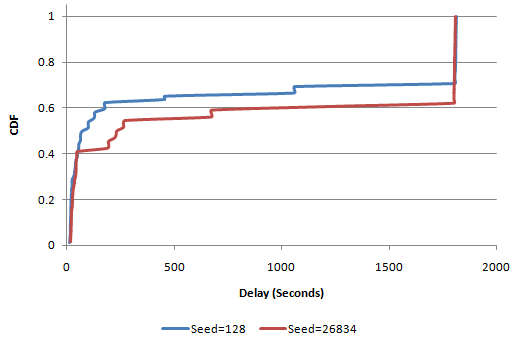
\includegraphics[width=0.8\textwidth]{images/result_delay_sim1byseed_mc3}
    \caption{Delay - Simulation 1 (1 Ferry, 1 Gateway), Memory Capacity of 3}
    \label{fig:result_delay_sim1byseed_mc3}
\end{figure}

\begin{figure}[htbp]
    \centering
    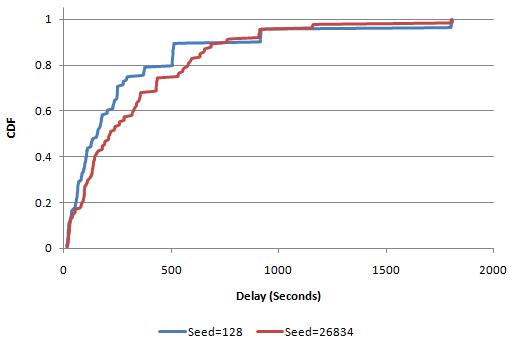
\includegraphics[width=0.8\textwidth]{images/result_delay_sim1byseed_mc30}
    \caption{Delay - Simulation 1 (1 Ferry, 1 Gateway), Memory Capacity of 30}
    \label{fig:result_delay_sim1byseed_mc30}
\end{figure}

\subsection{Simulation 2}

Figures \ref{fig:result_delay_sim2byseed_mc3} and \ref{fig:result_delay_sim2byseed_mc30} show the delay for simulation 2 with memory limits of 3 and 30 updates imposed by the ferries respectively.
As in section \ref{sec:results_success_s2}, randomness (as distinguished between the two seed values) has less effect on the output than simulation 1.
Comparing the memory constrained cases between simulations (figures \ref{fig:result_delay_sim1byseed_mc3} and \ref{fig:result_delay_sim2byseed_mc3}), it is clear that the second simulation has reduced delay and increased success rate.
It can be seen from figure \ref{fig:result_delay_sim2byseed_mc30} that 90\% of updates have a delay of approximately 300 seconds when memory is not constrained.

\begin{figure}[htbp]
    \centering
    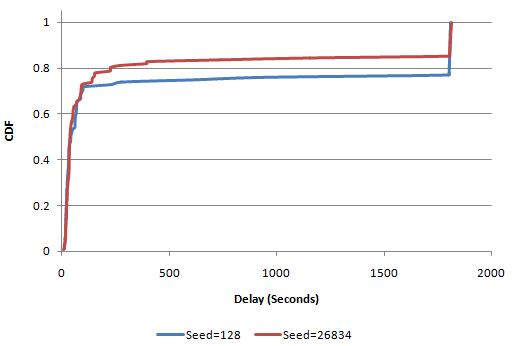
\includegraphics[width=0.8\textwidth]{images/result_delay_sim2byseed_mc3}
    \caption{Delay - Simulation 2 (2 Ferries, 2 Gateways), Memory Capacity of 3}
    \label{fig:result_delay_sim2byseed_mc3}
\end{figure}


\begin{figure}[htbp]
    \centering
    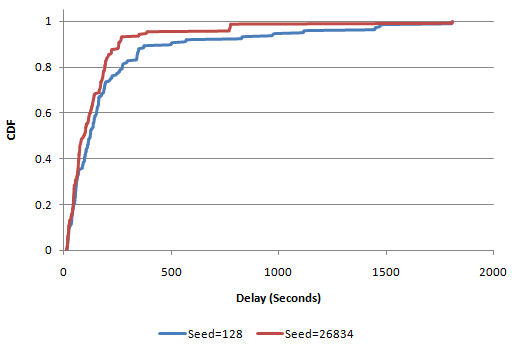
\includegraphics[width=0.8\textwidth]{images/result_delay_sim2byseed_mc30}
    \caption{Delay - Simulation 2 (2 Ferries, 2 Gateways), Memory Capacity of 30}
    \label{fig:result_delay_sim2byseed_mc30}
\end{figure}

\subsection{Comparison of Simulation}

Figures \ref{fig:result_delay_both_128_mc30} and \ref{fig:result_delay_both_128_mc5} provide a comparison of delay between the two scenarios.
It can be seen that the second scenario, with an additional ferry and gateway, has significantly reduced average delay.
Furthermore, very few updates take longer than approximately 300 seconds to reach the gateway.
When ferry memory capacity is limited to 5 updates, the additional ferry and gateway is seen to increase the probability updates are received in a timely manner.

\begin{figure}[htbp]
    \centering
    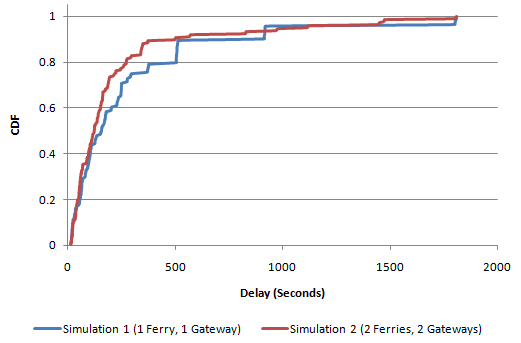
\includegraphics[width=0.8\textwidth]{images/result_delay_both_128_mc30}
    \caption{Delay - Simulation 1 and 2, Memory Capacity of 30, Seed of 26834}
    \label{fig:result_delay_both_128_mc30}
\end{figure}


\begin{figure}[htbp]
    \centering
    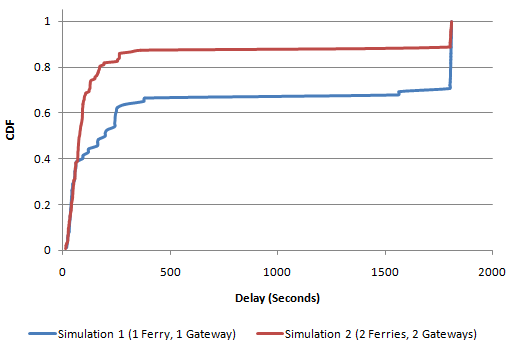
\includegraphics[width=0.8\textwidth]{images/result_delay_both_128_mc5}
    \caption{Delay - Simulation 1 and 2, Memory Capacity of 5, Seed of 128}
    \label{fig:result_delay_both_128_mc5}
\end{figure}